%\title{LaTeX Portrait Poster Template}
%%%%%%%%%%%%%%%%%%%%%%%%%%%%%%%%%%%%%%%%%
% a0poster Portrait Poster
% LaTeX Template
% Version 1.0 (22/06/13)
%
% The a0poster class was created by:
% Gerlinde Kettl and Matthias Weiser (tex@kettl.de)
% 
% Adapter by Jens Buysse for Hogeschool Gent
% This template has been downloaded from:
% http://www.LaTeXTemplates.com
%
% License:
% CC BY-NC-SA 3.0 (http://creativecommons.org/licenses/by-nc-sa/3.0/)
%
%%%%%%%%%%%%%%%%%%%%%%%%%%%%%%%%%%%%%%%%%

%----------------------------------------------------------------------------------------
%	PACKAGES AND OTHER DOCUMENT CONFIGURATIONS
%----------------------------------------------------------------------------------------

\documentclass[a0,portrait]{a0poster}

\usepackage{multicol} % This is so we can have multiple columns of text side-by-side
\columnsep=100pt % This is the amount of white space between the columns in the poster
\columnseprule=3pt % This is the thickness of the black line between the columns in the poster

\usepackage[svgnames]{xcolor} % Specify colors by their 'svgnames', for a full list of all colors available see here: http://www.latextemplates.com/svgnames-colors

\usepackage{times} % Use the times font
%\usepackage{palatino} % Uncomment to use the Palatino font

\usepackage{graphicx} % Required for including images
\graphicspath{{figures/}} % Location of the graphics files
\usepackage{booktabs} % Top and bottom rules for table
\usepackage[font=small,labelfont=bf]{caption} % Required for specifying captions to tables and figures
\usepackage{amsfonts, amsmath, amsthm, amssymb} % For math fonts, symbols and environments
\usepackage{wrapfig} % Allows wrapping text around tables and figures
\usepackage[export]{adjustbox}

\begin{document}

%----------------------------------------------------------------------------------------
%	POSTER HEADER 
%----------------------------------------------------------------------------------------

% The header is divided into two boxes:
% The first is 75% wide and houses the title, subtitle, names, university/organization and contact information
% The second is 25% wide and houses a logo for your university/organization or a photo of you
% The widths of these boxes can be easily edited to accommodate your content as you see fit

\begin{minipage}[t]{0.75\linewidth}
\VeryHuge \color{HoGentAccent1} \textbf{Studie naar de performantie-impact van Spectre/Meltdown patches op Linux voor een typische workload van een webserver} \color{Black}\\ % Title
%\Huge\textit{Ondertitel (eventueel)}\\[2.4cm] % Subtitle
\huge \textbf{Willems Karel, Bert Van Vreckem, Karine Van Driessche}\\[0.5cm] % Author(s)
\huge Hogeschool Gent, Valentin Vaerwyckweg 1, 9000 Gent\\[0.4cm] % University/organization
\Large \texttt{karel.willems.u7999@student.hogent.be} \\
\end{minipage}
%
\begin{minipage}[t]{0.25\linewidth}

\includegraphics[width=13cm,right]{figures/HG-woordmerk.jpg} 

\end{minipage}

\vspace{1cm} % A bit of extra whitespace between the header and poster content

%----------------------------------------------------------------------------------------

\begin{multicols}{2} % This is how many columns your poster will be broken into, a portrait poster is generally split into 2 columns

%----------------------------------------------------------------------------------------
%	ABSTRACT
%----------------------------------------------------------------------------------------

\color{HoGentAccent1} % Navy color for the abstract

\begin{abstract}
Dit werk is een studie van het performantieverschil van de Meltdown en Spectre patches op een Linux webserver.
Om dit uit te testen werd er met Vagrant en Ansible een testopstelling opgezet, om gemakkelijk resultaten te genereren.
Het resultaat is data van een aantal benchmark en monitoring tools.
Aan de hand van t-testen worden de resultaten onderzocht, en er wordt gezien of ze statistisch significant zijn.

In deze bachelorproef vind je achtergrond over hoe de Spectre/Meltdown aanvallen werken, en hoe risicobeperkende maatregelen de performantie kunnen be\"invloeden.
De resultaten duiden aan dat in de meeste applicaties er een significant verschil is.
Eerst werd er gezien of het processorgebruik tijdens een normale werklast veel verschilt.

Het antwoord was duidelijk, met een verschil van 18 procent.
De volgende test was op het vlak van responstijd, het verschil was hier redelijk, met 5 procent.
Redis, een in-memory database verloor maar 3 procent over allerlei andere testen.

Deze bachelorproef bevestigt dat de patches wel degelijk performantieverlies met zich meebrengen. 
Het performantieverlies voor een webserver is significant, doch niet rampzalig.
Dit is belangrijk voor webmasters die zich afvragen of ze nu al dan niet meer rekenkracht nodig hebben. De belangrijkste impact zal zijn op werkelijk grootschalige omgevingen zoals cloud-providers, waar zelfs een toename van een paar procenten van de belasting, extra hardware vereist.

De vraag is of de patches nog veel verbeterd kunnen worden, en wat de impact is op het vlak van energieverbruik, dat ook belangrijk is voor cloud-providers.

\end{abstract}
%----------------------------------------------------------------------------------------
%	INTRODUCTION
%----------------------------------------------------------------------------------------

\color{HoGentAccent1} 
\section*{Introductie}
\color{black}
\color{black}
Spectre en Meltdown zijn bugs op het vlak van beveiliging dat bestaan in apparaten van de afgelopen 20 jaar.
Redhat rapporteert dat Meltdown en Spectre tezamen een impact van 0 tot 19 procent
heeft. Applicaties die vaak systeemoproepen doen zullen meer prestatieverlies hebben.\newline
De 9de generatie Intel ’Ice Lake’ processors zullen hardwarematige oplossingen hebben, maar deze zijn beschikbaar in 2019.
\newline
Nieuwe processors zijn echter duur, dus het is niet vanzelfsprekend om nieuwe te kopen.\newline
Wie in de markt is voor een nieuwe processor, kan nu kopen of tot 2019 wachten. Deze studie moet duidelijke resultaten geven of er een drastisch verschil is voor webapplicaties.\newline De onderzoeksvraag die moet beantwoord worden in deze studie is:\newline\newline
''Is er een groot performantieverschil met de Spectre/Meltdown patches op een Linux
webserver``
%----------------------------------------------------------------------------------------
%	GEOLOGY
%----------------------------------------------------------------------------------------

\color{Black} % DarkSlateGray color for the rest of the content
\color{HoGentAccent1} 
\section*{Experimenten}
\color{black}
Het vergelijken wordt vooraf gegaan door een t-test, die duidelijk zal maken of het verschil statistisch significant is. Hiervoor wordt de alpha-waarde als standaard genomen: 0,05. De p-waarde moet kleiner zijn als de alpha-waarde, om met zekerheid te zeggen dat de meetresultaten betrouwbaar zijn.
\newline\newline
\noindent\textbf{CPU gebruik.}
De belasting werd gegenereerd door autobench met 40 verzoeken per seconde voor een totaal van 4500 verzoeken. Het CPU gebruik werd opgeslaan elke seconde voor 90 seconden met vmstat. Het vmstat commando wordt naar de webservers gedelegeerd.
\newline\newline
\noindent\textbf{Responstijd.} Responstijd werd verkregen door de latentie te berekenen voor een bepaald aantal van gelijktijdige verbindingen.De gelijktijdige verbindingen lopen uiteen van 20 tot 240 met stappen van 2. De gebruikte tool heet ’autobench’.
\newline\newline
\noindent\textbf{Redis.} De resultaten van redis (een 'in memory' database) zijn berekend met ’redis-benchmark’, een hulpprogramma opgenomen in Redis.Het systeem met patches verliest 3,4\% performantie.
De doorvoersnelheid werd met dezelfde methode berekend als de responstijd (20 tot 240 gelijktijdige verbindingen met stappen van 2).
\newline\newline
\textbf{Doorvoersnelheid.}
Het systeem met de patches heeft een doorvoersnelheid van 54 verzoeken per seconde, het
systeem zonder patches een doorvoersnelheid van 58 . Dit is een verlies van 7 procent.


\color{HoGentAccent1} 
\section*{Sectie met figuur}
\color{black}


\begin{center}\vspace{1cm}
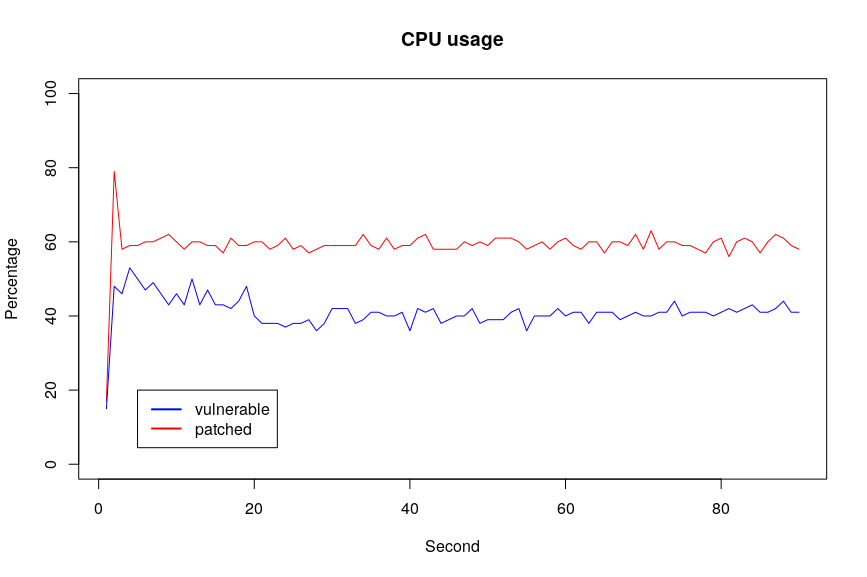
\includegraphics[width=1.0\linewidth]{cpu_usage.png}
\captionof{figure}{\color{HoGentAccent5} CPU gebruik}
\end{center}\vspace{1cm}

%------------------------------------------------



\color{HoGentAccent1} 
\section*{Conclusies}
\color{black}
Uit het onderzoek bleek dat de Meltdown/Spectre patches wel degelijk een performantieverlies introduceren. Vooral processor verbruik stijgt. Voor een webserver is het
performantieverlies niet drastisch, maar bij grootschalige servers kan 5\% al zeer impactvol zijn.\newline
In het begin veroorzaakten de patches veel problemen, zoals spontane reboots maar ze zijn nu veel verbeterd met betrekking tot stabiliteit en performantie. De doorvoersnelheid van een normale webserver verliest maar 7 procent. Dat is veel minder dan eerst gedacht, sommigen voorspelden rond de 30 procent.\newline
Waar het onderzoek geen definitief antwoord op kan geven is de performantie van redis, alhoewel er weinig verschil op zit. Als we naar de responstijd zien, is de server nog perfect bruikbaar met een stijging van 1 milliseconde (van 14ms naar 15ms).
%----------------------------------------------------------------------------------------
%	FORTHCOMING RESEARCH
%----------------------------------------------------------------------------------------
\color{HoGentAccent1} 
\section*{Toekomstig onderzoek}
\color{black}

De vraag is of de patches nog veel verbeterd kunnen worden, en wat de impact is op het
vlak van energieverbruik, dat ook belangrijk is voor cloud-providers.


%----------------------------------------------------------------------------------------

\end{multicols}
\end{document}
